\song{Holubí dům (Jiří Schelinger)}
\begin{multicols}{2}
%\re{}(capo 1)

\ve{}
\ch{Em D}Zpívám \ch{C}ptákům a \ch{Hm7}zvlášť holu\ch{Em}bům,\\
stá\ch{D}val v \ch{C}{ú}dolí \ch{Hm7}mém starý \ch{Em}dům.\\
\ch{G}Ptá\ch{D}ků \ch{G}houf \ch{G}zalé\ch{D}tal ke kro\ch{G}vům,\\
\ch{Em}měl \ch{D}jsem \ch{Cmaj7}rád holu\ch{Hm7}bích křídel \ch{Em}{š}um.

\ve{}
Vlídná dívka jim házela hrách,\\
mávání perutí víří prach.\\
Ptáci krouží a neznají strach,\\
měl jsem rád starý dům, jeho práh.

\cho{}
Hledám \ch{Am}dům holu\ch{D}bí,\\
kdopak z \ch{G}vás cestu \ch{Em}ví,\\
míval \ch{Ami}stáj roube\ch{D}nou, bílý \ch{G}{š}tít.\\
Kde je \ch{Am}dům holu\ch{D}bí a ta \ch{G}dívka kde \ch{Em}spí?\\
Vždyť to \ch{Am}ví, že jsem \ch{Hm7}chtěl pro ni \ch{Em}{ž}ít.

\ve{}
Sdílný déšť vypráví okapům,\\
bláhový, kdo hledá tenhle dům.\\
Odrůstáš chlapeckým střevícům,\\
neslyšíš holubích křídel šum.

\ve{}
Nabízej úplatou cokoli,\\
nepojíš cukrových homolí.\\
Můžeš mít třeba zrak sokolí,\\
nespatříš ztracené údolí.

\re{*}
\ch{Em D}Zpívám \ch{C}ptákům a \ch{Hm7}zvlášť holu\ch{Em}bům,\\
stá\ch{D}val v \ch{Cmaj}{ú}dolí \ch{Hm7}mém starý \ch{Em}dům.

\columnbreak
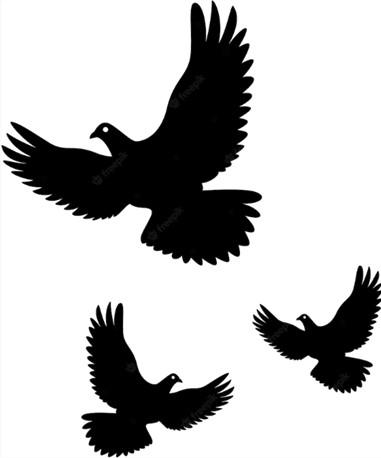
\includegraphics[width = \columnwidth]{images/holubi_dum.jpg}
\end{multicols}
\esong{}